\documentclass{article}
\usepackage[english]{babel}
\usepackage[letterpaper,top=2cm,bottom=2cm,left=3cm,right=3cm]{geometry}
\usepackage{amsmath}
\usepackage{booktabs}
\usepackage{graphicx}
\usepackage{float}
\usepackage{tikz}
\usetikzlibrary{arrows.meta,positioning,shapes.geometric}
\usepackage[colorlinks=true,allcolors=blue]{hyperref}
\usepackage[sort&compress,round,semicolon,authoryear]{natbib}
\usepackage[figurename=Fig.,labelfont=bf,labelsep=period]{caption}

\title{When Braess Paradox Runs Induced Demand in Reverse}
\author{David Levinson}
\date{\today}

\begin{document}
\maketitle

\begin{abstract}
Induced demand is usually stated as lower generalized cost producing more travel. A Braess network can reverse that comparative static: an added link may raise user-equilibrium cost, and elastic demand then falls. With downward-sloping inverse demand, reduced demand follows from the Braess cost increase. I show this in a canonical four-node network with linear link costs and inverse demand. In the default case, the added link raises elastic equilibrium cost from 64.29 to 72.00 and reduces demand from 3.86 to 3.60. The reported 572-point sweep maps the Braess region; no sign-inconsistent cells appear.
\end{abstract}

\textit{Keywords:} Braess paradox, induced demand, elastic demand, user equilibrium, network design

\section{Questions}

Induced demand is commonly described as the response of travel to lower generalized cost. Lee, Klein, and Camus define induced traffic as movement along a travel-demand curve, where price includes travel time and other user costs \citep{lee1999induced}. The same demand curve has a reverse implication: if generalized cost rises, equilibrium travel should fall. Empirical studies of capacity reduction describe related outcomes as reduced, suppressed, or disappearing traffic \citep{goodwin1998capacity,cairns2002disappearing,behrens2004capacity,zhu2010i35w}.

Braess paradox supplies a network mechanism for this reverse case. Under user equilibrium, adding a link can increase travelers' costs rather than reduce them \citep{braess1968paradoxon,braess2005paradox,murchland1970braess,yang1998capacity}. Prior work gives tests for equilibrium cost changes under demand changes and added routes \citep{dafermos1984paradoxes}, shows that the paradox can disappear at higher demand when the Braess link is no longer used \citep{nagurney2010negation}, and examines elastic-demand traffic paradoxes \citep{hallefjord1994traffic,tu2019traffic,nagurney2020braess}. This note connects those strands by classifying when an added Braess link produces reduced demand. The contribution is conceptual and classificatory, not a general network-design theorem. I ask two questions:

\begin{enumerate}
  \item In a transparent canonical Braess network, when does an added link produce reduced demand under a downward-sloping inverse-demand curve?
  \item Over a small parameter grid, where does the added link raise equilibrium cost, thereby implying reduced demand?
\end{enumerate}

\section{Methods}

The model is the canonical directed four-node Braess network with one origin-destination pair. Link 1 runs from Origin to Upper, link 3 from Upper to Destination, link 2 from Origin to Lower, and link 4 from Lower to Destination. Link 5 is the candidate Upper-to-Lower connector. The upper path is links 1--3, the lower path is links 2--4, and the added-link path is links 1--5--4. The default link performance functions are
\[
t_1(x)=10x,\quad t_4(x)=10x,\quad t_2(x)=45,\quad t_3(x)=45,\quad t_5(x)=0,
\]
with fixed demand \(q=6\). The candidate link is solved both off and on.

For each scenario, the model enumerates all simple origin-destination paths and solves static Wardrop user equilibrium by Method of Successive Averages \citep{sheffi1985urban}. At each iteration, link costs are evaluated from current flows, all demand is assigned to the current shortest path, and path flows are averaged using the diminishing step size \(1/k\). This averaging is the convergence device: it damps path switching. The stopping tolerance is \(10^{-6}\) after at least five iterations, with a 120-iteration maximum. For the nonnegative affine and Bureau of Public Roads-style separable link costs used here, this is the standard monotone user-equilibrium setting. I do not claim convergence for arbitrary non-monotone user-edited cost functions.

Elastic demand uses inverse demand
\[
C(q)=A-Bq.
\]
The default elastic case sets \(A=180\) and \(B=30\), so the zero-cost demand intercept remains \(A/B=6\). Computationally, the model uses an outer bisection on \(q\); for each trial quantity, it solves Wardrop equilibrium and compares the resulting network cost with \(A-Bq\). Bisection is appropriate when \(c(q)-C(q)\) is monotone over the bracket, as it is for the downward-sloping inverse demand and monotone link costs used in the reported sweeps. Reported elastic costs are network costs \(c(q^*)\); they equal \(C(q^*)\) at the exact fixed point, apart from numerical tolerance and rounding. Conceptually, the elastic-demand solution is a fixed point where route flows and demand agree simultaneously: \(c(q^*)=C(q^*)\) (Fig.~\ref{fig:feedback}).

\begin{table}[H]
  \centering
  \small
  \begin{tabular}{ll}
    \toprule
    Symbol & Definition \\
    \midrule
    \(x\) & Flow on a link. \\
    \(t_i(x)\) & Travel time on link \(i\) when its flow is \(x\). \\
    \(q\) & Origin-destination demand in a fixed-demand or trial elastic-demand solve. \\
    \(q^*\) & Elastic-demand equilibrium quantity. \\
    \(C(q)\) & Inverse-demand generalized cost, or willingness to pay, at quantity \(q\). \\
    \(A\) & Zero-trip willingness-to-pay intercept in \(C(q)=A-Bq\). \\
    \(B\) & Inverse-demand slope; larger \(B\) means willingness to pay falls faster with \(q\). \\
    \(c(q)\) & Wardrop equilibrium origin-destination cost after assigning quantity \(q\). \\
    \(s\) & Scenario index, either candidate link off or candidate link on. \\
    \(c_s(q_s^*)\) & Elastic equilibrium network cost in scenario \(s\). \\
    \(c_{\mathrm{on}}, c_{\mathrm{off}}\) & Equilibrium costs with the candidate link on and off. \\
    \(q_{\mathrm{on}}, q_{\mathrm{off}}\) & Elastic equilibrium quantities with the candidate link on and off. \\
    \(b\) & Congestion coefficient on the swept variable-cost links. \\
    \bottomrule
  \end{tabular}
  \caption{Nomenclature for the model equations and comparison tests.}
  \label{tab:nomenclature}
\end{table}

\begin{figure}[H]
  \centering
  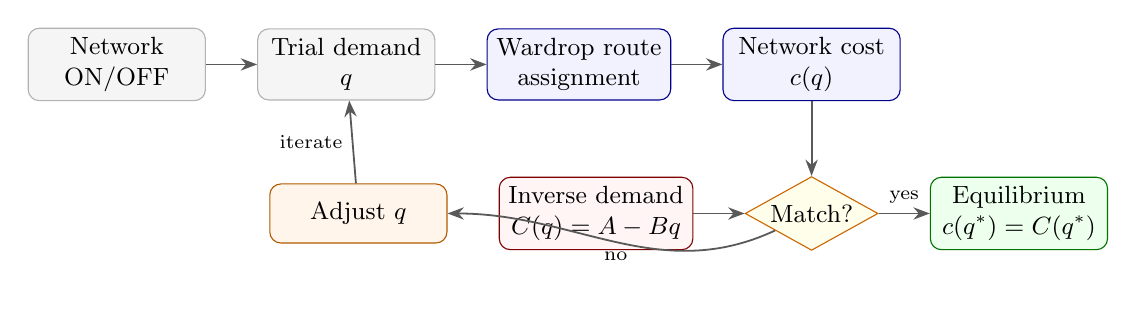
\begin{tikzpicture}[
    node distance=0.85cm and 0.65cm,
    >=Stealth,
    box/.style={draw, rounded corners, align=center, minimum width=2.25cm, minimum height=0.75cm, font=\small},
    network/.style={box, fill=gray!8, draw=gray!60},
    assignment/.style={box, fill=blue!5, draw=blue!55!black},
    demand/.style={box, fill=red!4, draw=red!50!black},
    adjust/.style={box, fill=orange!8, draw=orange!70!black},
    equilibrium/.style={box, fill=green!7, draw=green!45!black},
    decision/.style={draw, diamond, aspect=1.8, align=center, fill=yellow!8, draw=orange!80!black, inner sep=1.2pt, font=\small},
    arrow/.style={->, line width=0.65pt, draw=black!65}
  ]
    \node[network] (network) {Network\\ON/OFF};
    \node[network, right=of network] (trial) {Trial demand\\\(q\)};
    \node[assignment, right=of trial] (wardrop) {Wardrop route\\assignment};
    \node[assignment, right=of wardrop] (cost) {Network cost\\\(c(q)\)};
    \node[decision, below=0.95cm of cost] (compare) {Match?};
    \node[demand, left=of compare] (inverse) {Inverse demand\\\(C(q)=A-Bq\)};
    \node[equilibrium, right=of compare] (equilibrium) {Equilibrium\\\(c(q^*)=C(q^*)\)};
    \node[adjust, left=of inverse] (adjust) {Adjust \(q\)};

    \draw[arrow] (network) -- (trial);
    \draw[arrow] (trial) -- (wardrop);
    \draw[arrow] (wardrop) -- (cost);
    \draw[arrow] (cost) -- (compare);
    \draw[arrow] (inverse) -- (compare);
    \draw[arrow] (compare) -- node[above, font=\scriptsize] {yes} (equilibrium);
    \draw[arrow] (compare) to[out=205,in=0] node[below, font=\scriptsize] {no} (adjust);
    \draw[arrow] (adjust) -- node[left, font=\scriptsize] {iterate} (trial);
  \end{tikzpicture}
  \caption{Elastic-demand feedback. The numerical method iterates over trial quantities, but the object being solved is the fixed point where user-equilibrium generalized cost equals willingness to pay.}
  \label{fig:feedback}
\end{figure}

\noindent\textit{Sign implication.} For scenario \(s\in\{\mathrm{off},\mathrm{on}\}\), elastic equilibrium satisfies \(c_s(q_s^*)=C(q_s^*)\). If \(C\) is strictly decreasing and the added link raises elastic equilibrium cost, \(c_{\mathrm{on}}(q_{\mathrm{on}}^*)>c_{\mathrm{off}}(q_{\mathrm{off}}^*)\), then \(q_{\mathrm{on}}^*<q_{\mathrm{off}}^*\). Reduced demand is therefore the implication of the Braess cost increase, not a separate empirical regularity.

The Braess flag is \(c_{\mathrm{on}}-c_{\mathrm{off}}>10^{-5}\). The reported sweep varies \(A\in[90,270]\), \(B\in[15,45]\), and the coefficient \(b\) on links 1 and 4 over \(\{4,8,12,16\}\), for 572 grid points. The default \(b=10\) case is the illustrative example, not a grid point. The browser implementation, Braess Explorer, generated the numerical results and lets readers edit the network and demand curve.

\section{Findings}

The fixed-demand default reproduces the Braess paradox. Without the added link, equilibrium cost is 75.00. With the added link, equilibrium cost is 90.00, a 15.00-unit increase. Total travel time rises from 450.00 to 540.00.

The elastic-demand default converts the same network effect into reduced demand. With \(A=180\) and \(B=30\), the added link raises equilibrium cost from 64.29 to 72.00 and lowers equilibrium demand from 3.86 to 3.60 (Fig.~\ref{fig:default}). The result is the induced-demand comparative static with the network-cost sign reversed: the added link changes the network equilibrium cost relation, and demand adjusts until generalized cost equals willingness to pay.

\begin{figure}[H]
  \centering
  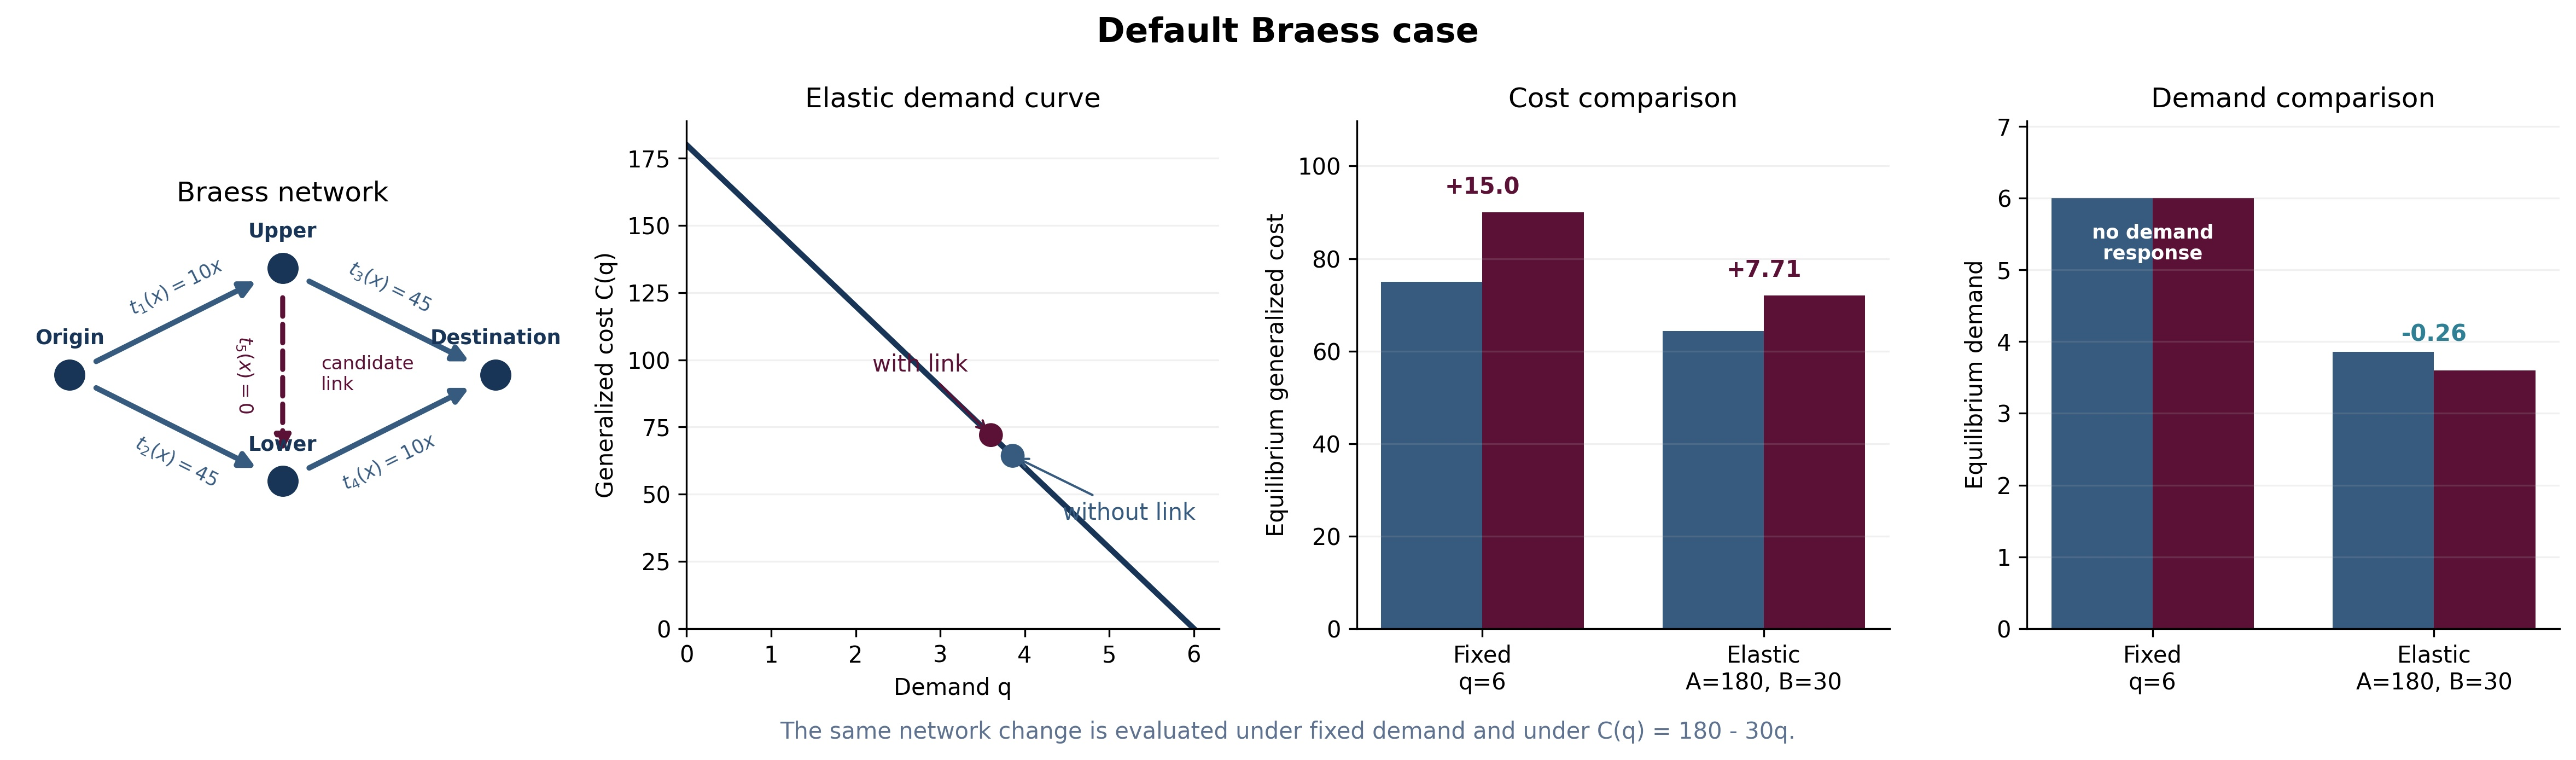
\includegraphics[width=\linewidth]{figures/figure-1-default-comparison.jpeg}
\caption{Default Braess comparison. The first panel shows the directed Braess network and link performance functions; the demand-curve panel places the OFF and ON elastic equilibria on \(C(q)\); the remaining panels compare cost and demand under fixed and elastic assumptions.}
  \label{fig:default}
\end{figure}

The outcome-space sweep maps where Braess occurs rather than testing whether reduced demand follows. In the reported A-B-\(b\) grid, the added link raises equilibrium cost in 317 of 572 cells (55.4\%). Demand is lower beyond tolerance in 277 cells and within demand-change tolerance in 40 boundary cells. Where the added link does not raise cost, demand usually increases; the 8 no-change cells are unused-link or tolerance-boundary cases. The two sign-inconsistent cases under a downward-sloping inverse-demand curve, Braess with increased demand and no Braess with reduced demand, have zero grid points (Table~\ref{tab:classes}; Fig.~\ref{fig:space}).

\begin{table}[H]
  \centering
  \begin{tabular}{lrr}
    \toprule
    Outcome in reported sweep & Grid points & Share \\
    \midrule
    BP; demand lower & 277 & 48.4\% \\
    BP; demand unchanged within tolerance & 40 & 7.0\% \\
    No BP; demand higher & 247 & 43.2\% \\
    No BP; demand unchanged within tolerance & 8 & 1.4\% \\
    Sign-inconsistent cases & 0 & 0.0\% \\
    \bottomrule
  \end{tabular}
  \caption{Classification of the 572-point elastic-demand outcome-space sweep. No-change rows are numerical-tolerance or unused-link boundary cases.}
  \label{tab:classes}
\end{table}

\begin{figure}[H]
  \centering
  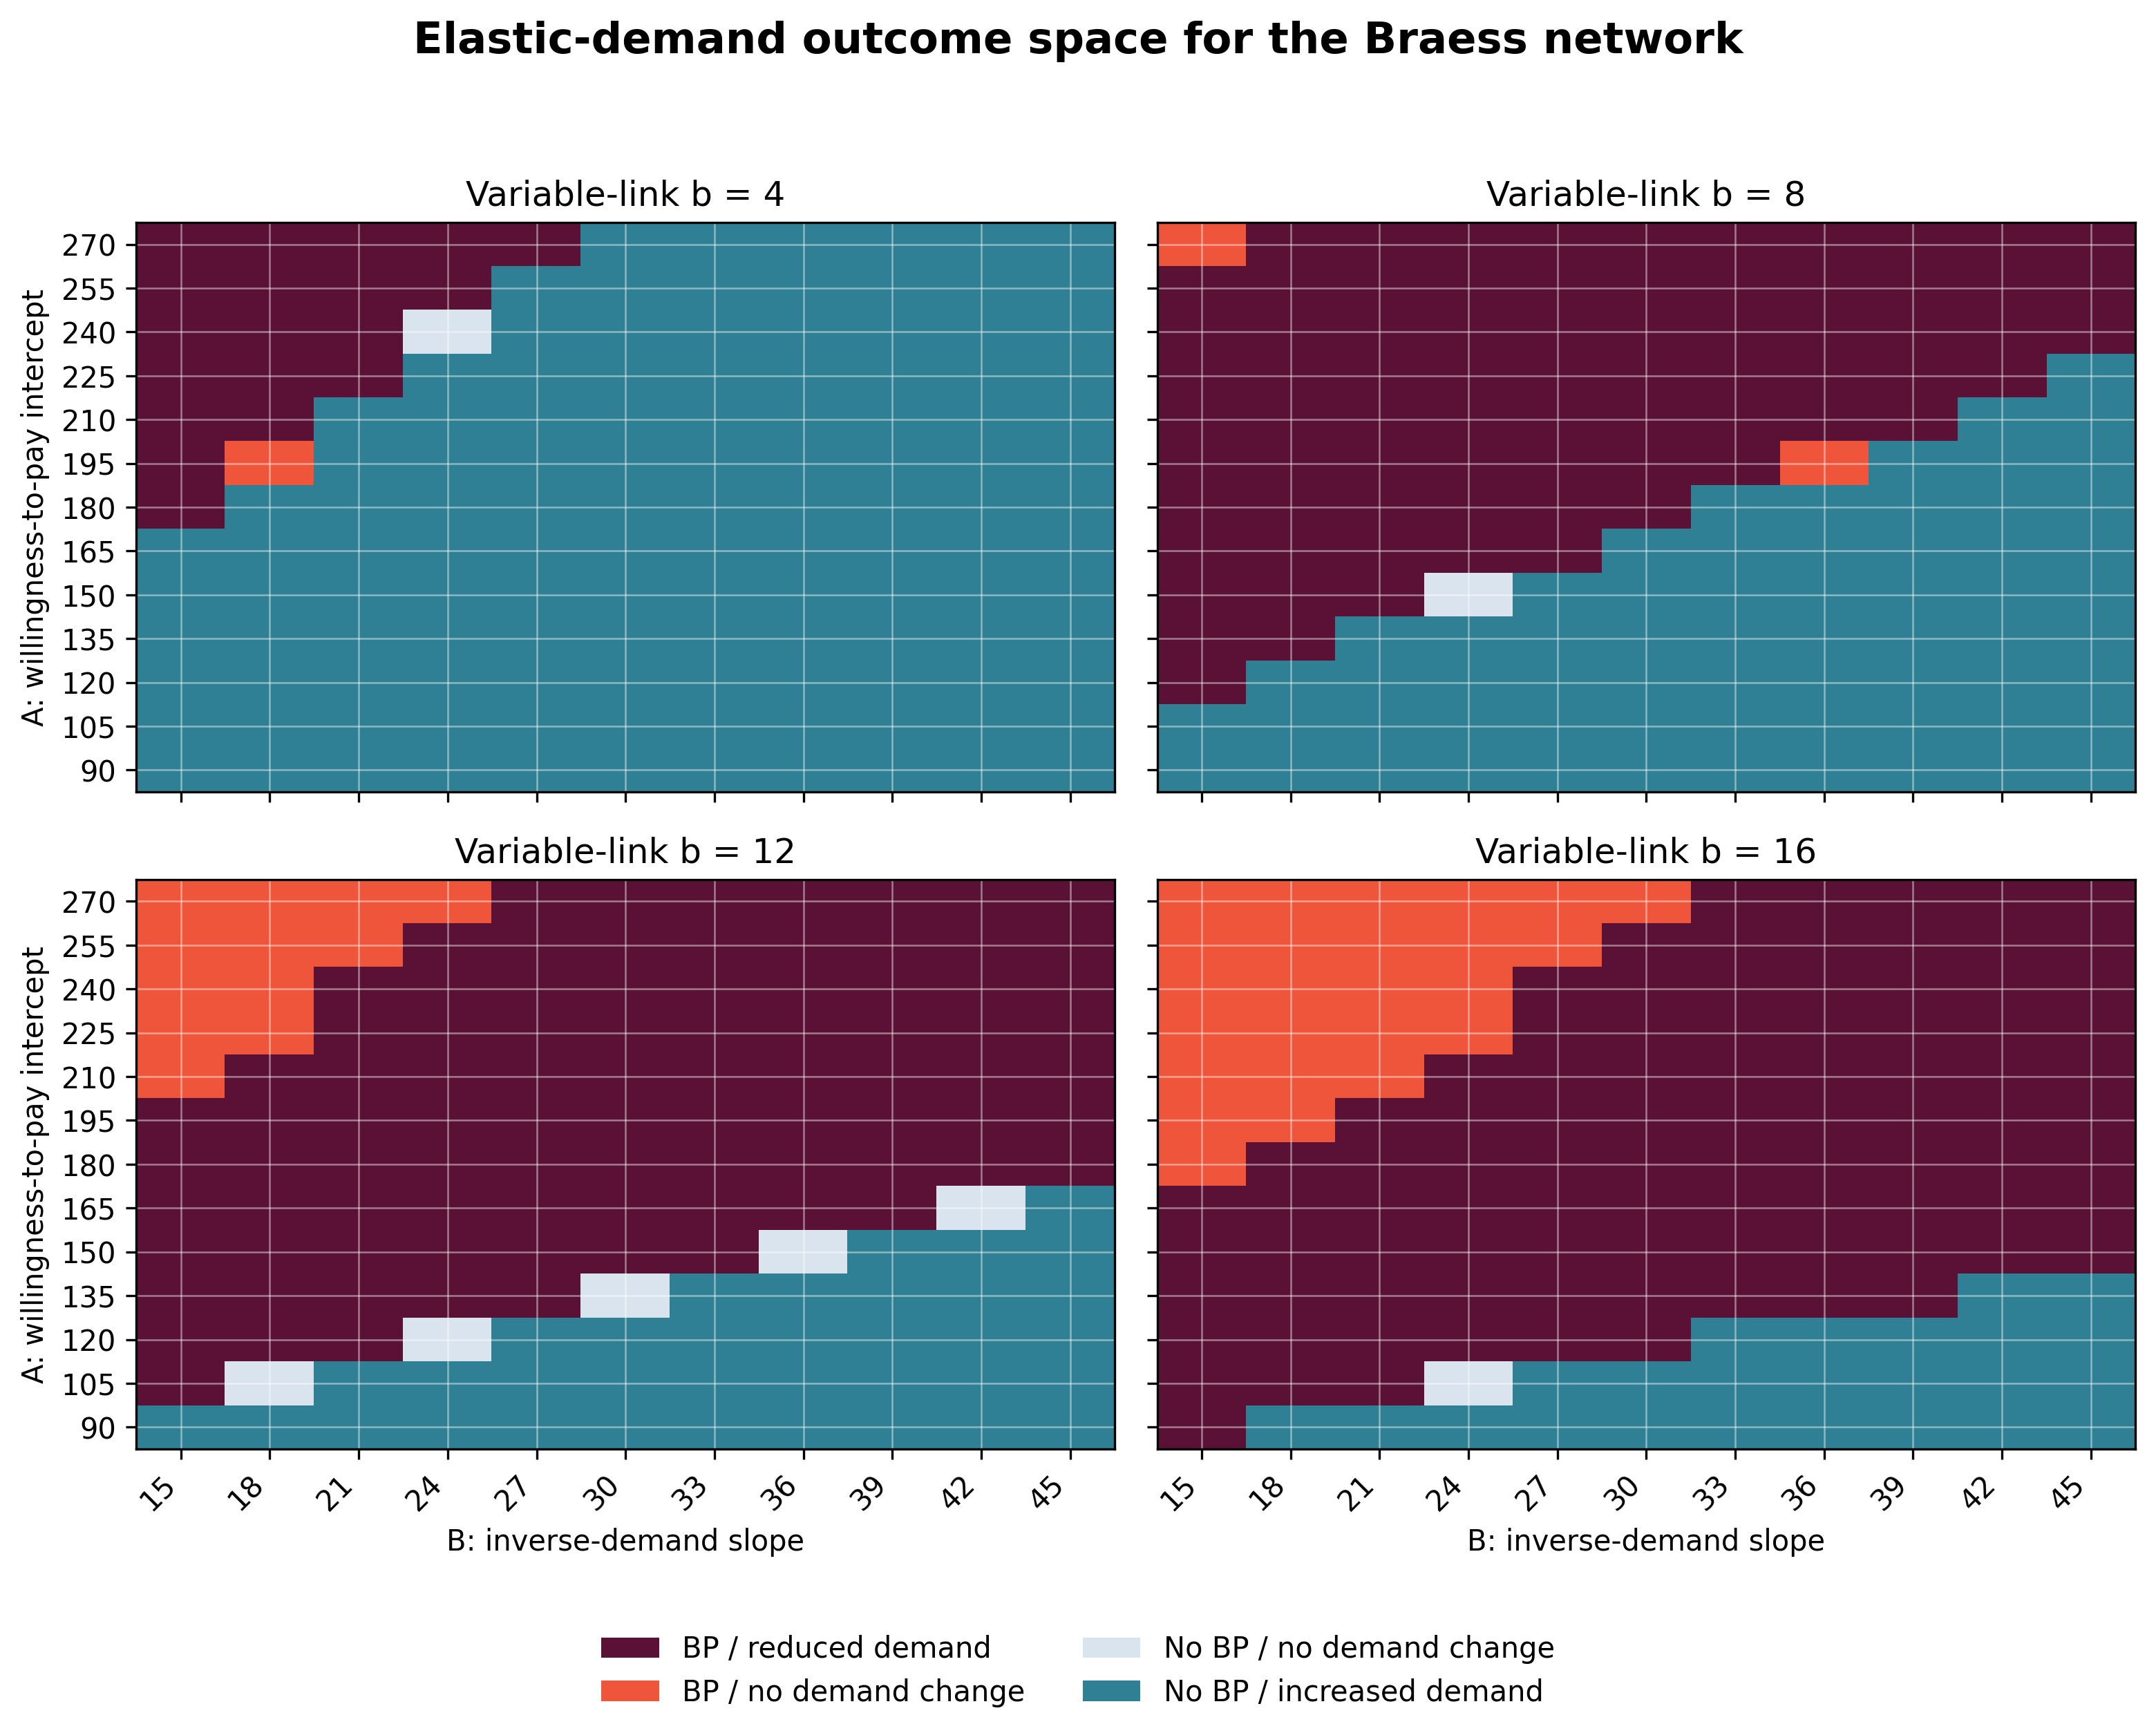
\includegraphics[width=\linewidth]{figures/figure-2-elastic-outcome-space.jpeg}
  \caption{Elastic-demand outcome space over inverse-demand intercept \(A\), inverse-demand slope \(B\), and variable-link coefficient \(b\).}
  \label{fig:space}
\end{figure}

The outcome map gives a compact diagnostic for interpreting added capacity under elastic demand. The ``No BP / increased demand'' class is the familiar induced-demand case: the added link does not worsen equilibrium cost and demand increases. The ``BP / reduced demand'' class is the reverse case: the added link worsens equilibrium cost through Braess paradox and demand falls. The same demand law appears in both regions; the network determines which sign is expressed.

\section*{Data Availability}

The Braess Explorer app, model code, export scripts, CSV files, and figures are at \url{https://github.com/dlevinson/braess-js}. The app runs entirely in the browser from \path{web/index.html}, allowing readers to edit the network, move the demand curve, rerun the default comparison, and export new sweep results. The main exported files are in the \path{findings-paper/data/} folder, and the manuscript figures are in \path{findings-paper/figures/}.

\bibliographystyle{chicago}
\bibliography{references}

\end{document}
